\documentclass{article}
\usepackage[utf8]{inputenc}

\usepackage{pgfplots}

\usepackage{csvsimple}

\pgfplotsset{compat=1.18}

\title{4 -- Convergence Plots and Tables}

\begin{document}
\maketitle

In the context of numerical methods, results should generally be presented
with both a clear plot and a table of values. Let's show a plot of relative
errors for each method, showing machine epsilon, and present a table of values.

We're using the \texttt{csvsimple} package to import CSV files

\section{Bisection}

Bisection method is the slowest out of the three methods. It converges
linearly, as the error halves each step. In the plot below it makes sense
that error looks linear on a log scale.

\subsection{Plot}

Here's a matplotlib plot, generated in Python, of the relative error of the
bisection method. The dotted red line is the machine epsilon. Any values lower
than this are meaningless, equivalent to random noise. Once the function
reaches machine epsilon, we consider the root found.

\begin{figure}
    \centering
    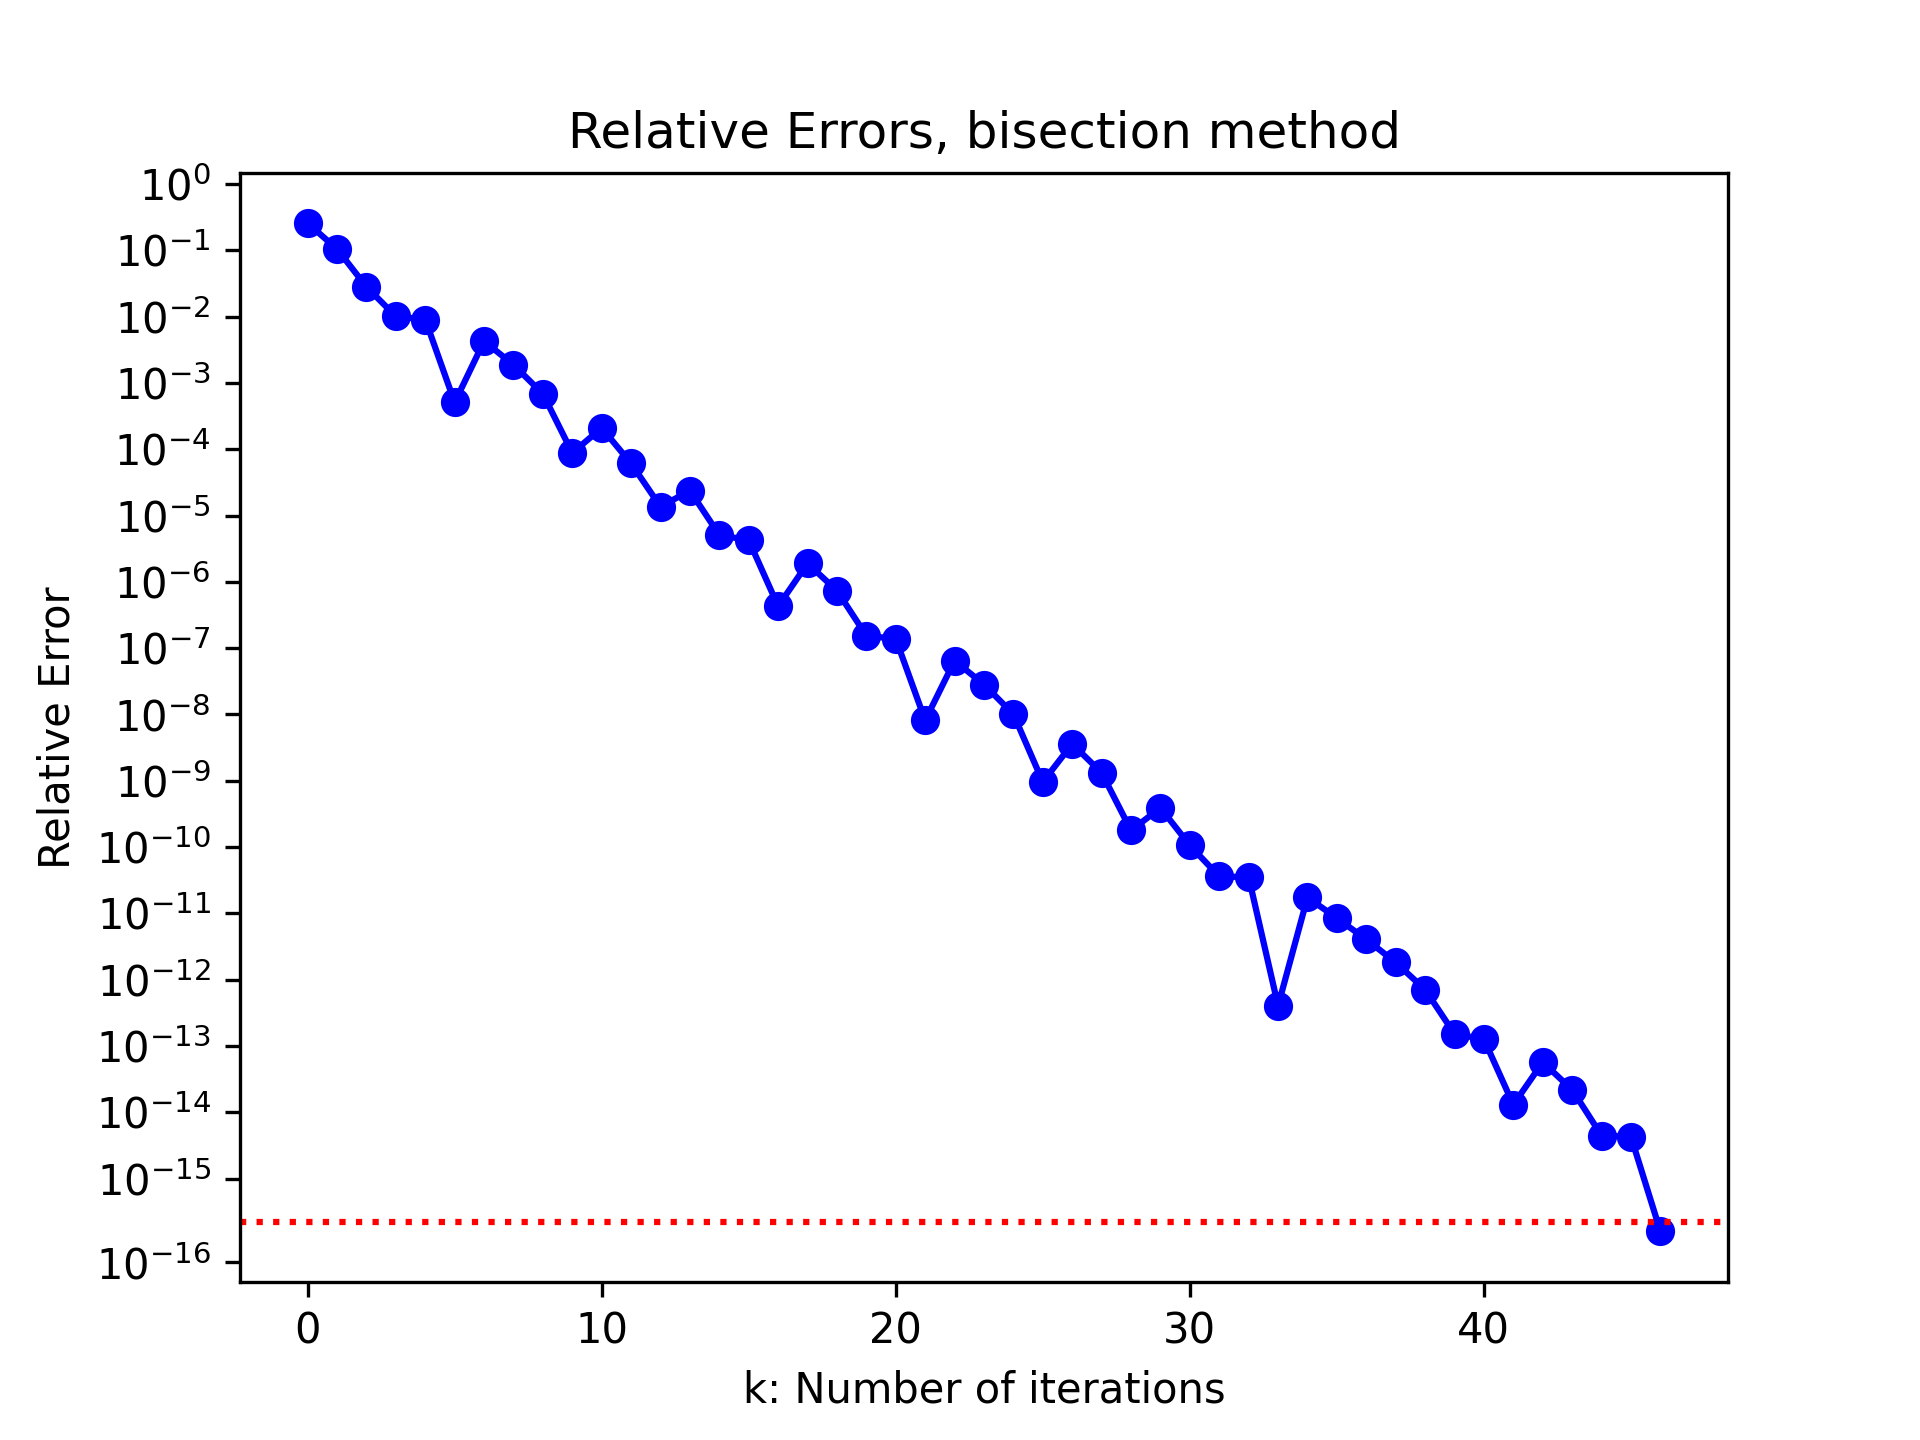
\includegraphics[scale=0.7]{./plots/bisectionrel.png}
    \caption {A matplotlib plot of the relative error of the Bisection method}
\end{figure}

\newpage

\subsection{Table (Ugly)}

Here's a directly imported table from a CSV file. Notice that the
columns aren't bolded, and the elements are left aligned. This
is bad practice for tables of numbers.

\newpage
\begin{figure}
    \centering
    \csvautotabular{./tables/bisectionrel.csv}
    \caption{Wow this table is too long}
\end{figure}

\subsection{Table (Nice)}

We can instead control how the table is rendered. Let's use
\LaTeX formatting for the math symbols.

\begin{figure}
    \centering
    \begin{tabular}{|r|r|r|r|}\hline%
    $k$ & $x$ & $f(x)$ & \bfseries Rel. Error\\\hline\hline
    \csvreader[
        late after line = \\\hline,
        ]{./tables/bisectionrel.csv}%
        {k=\k, x=\x, f=\f, relerror=\relerror}%
        {\k & \x & \f & \relerror}%
    \end{tabular}
    \caption{This table is still too long, but it does look better}
\end{figure}

\newpage


\section{Newton's}

Let's show the same convergence plots and tables for Newton's method.

\subsection{Plot}

\begin{figure}[h]
    \centering
    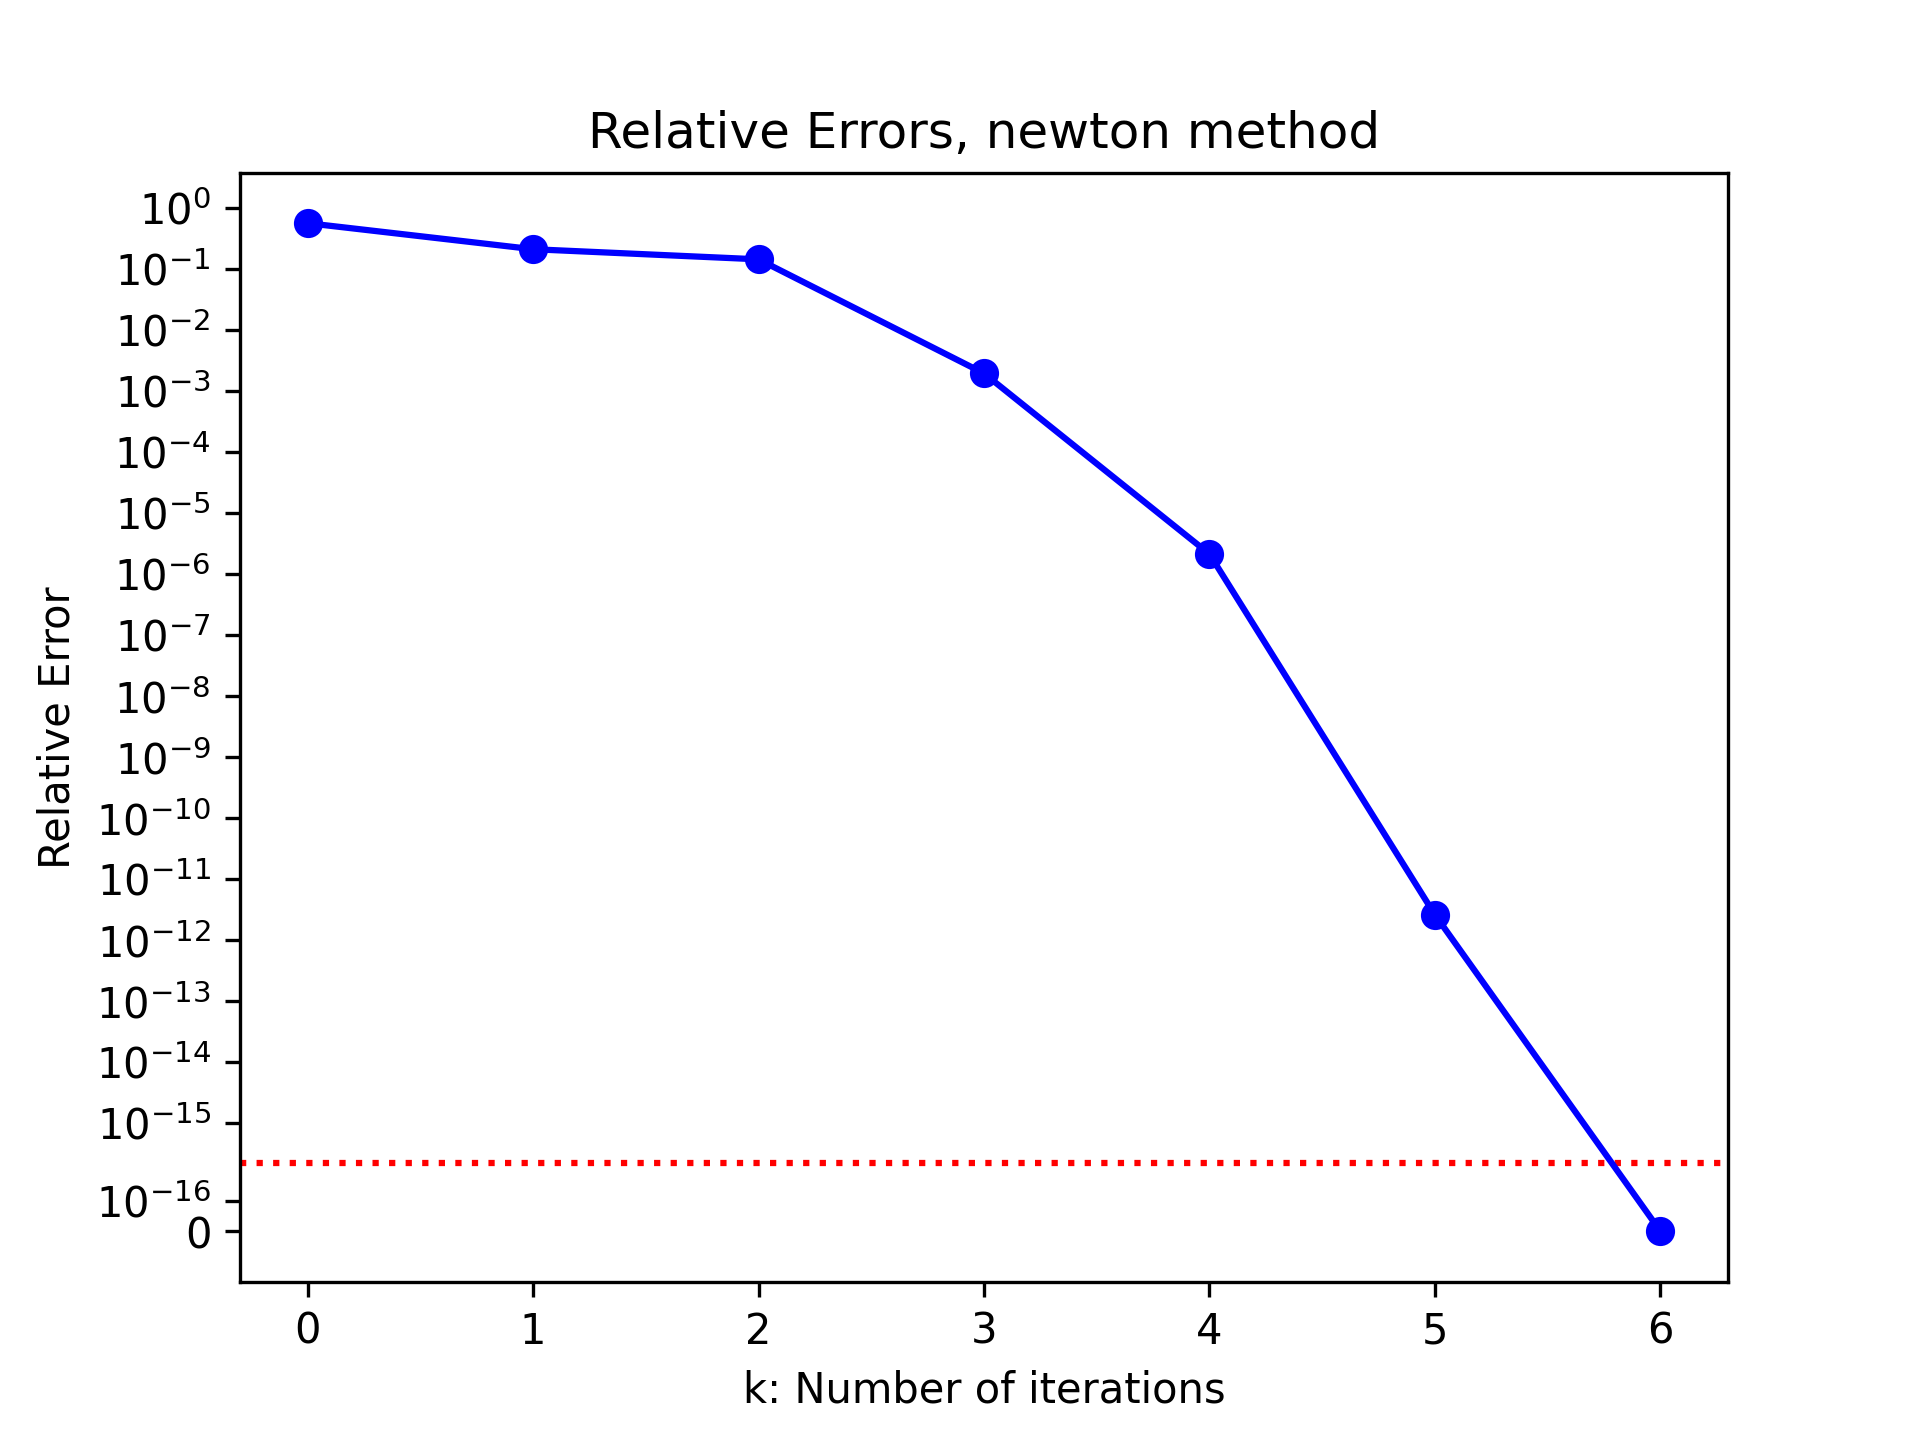
\includegraphics[scale=0.8]{./plots/newtonrel.png}
    \caption{A matplotlib plot of the relative error of Newton's method}
\end{figure}


\subsection{Table (Ugly)}

Notice that this table is a lot smaller than for the Bisection method.
This makes sense, as Newton's converges quadratically. At each step,
the number of zeros doubles.

\begin{figure}[h]
    \centering
    \csvautotabular{./tables/newtonrel.csv}
    \caption{A table of the relative error of Newton's method}
\end{figure}


\subsection{Table (Nice)}

Again, we can make it look better.

\begin{figure}[h]
    \centering
    \begin{tabular}{|r|r|r|r|}\hline%
    $k$ & $x_k$ & $f(x_k)$ & \bfseries Rel. Error\\\hline\hline
    \csvreader[
        late after line = \\\hline,
        ]{./tables/newtonrel.csv}%
        {k=\k, x=\x, f=\f, relerror=\relerror}%
        {\k & \x & \f & \relerror}%
    \end{tabular}
    \caption{A better looking table of the relative error of Newton's method}
\end{figure}

\newpage
\section{Secant}
For this function $f(x) = e^{-x} \sin(e^x)$, Secant and Newton perform similarly.
This function's derivative is not too expensive to calculate, it could be much worse.

\subsection{Plot}

Here's a matplotlib plot, generated in Python, of the relative error of the
secant method.

\begin{figure}[h]
    \centering
    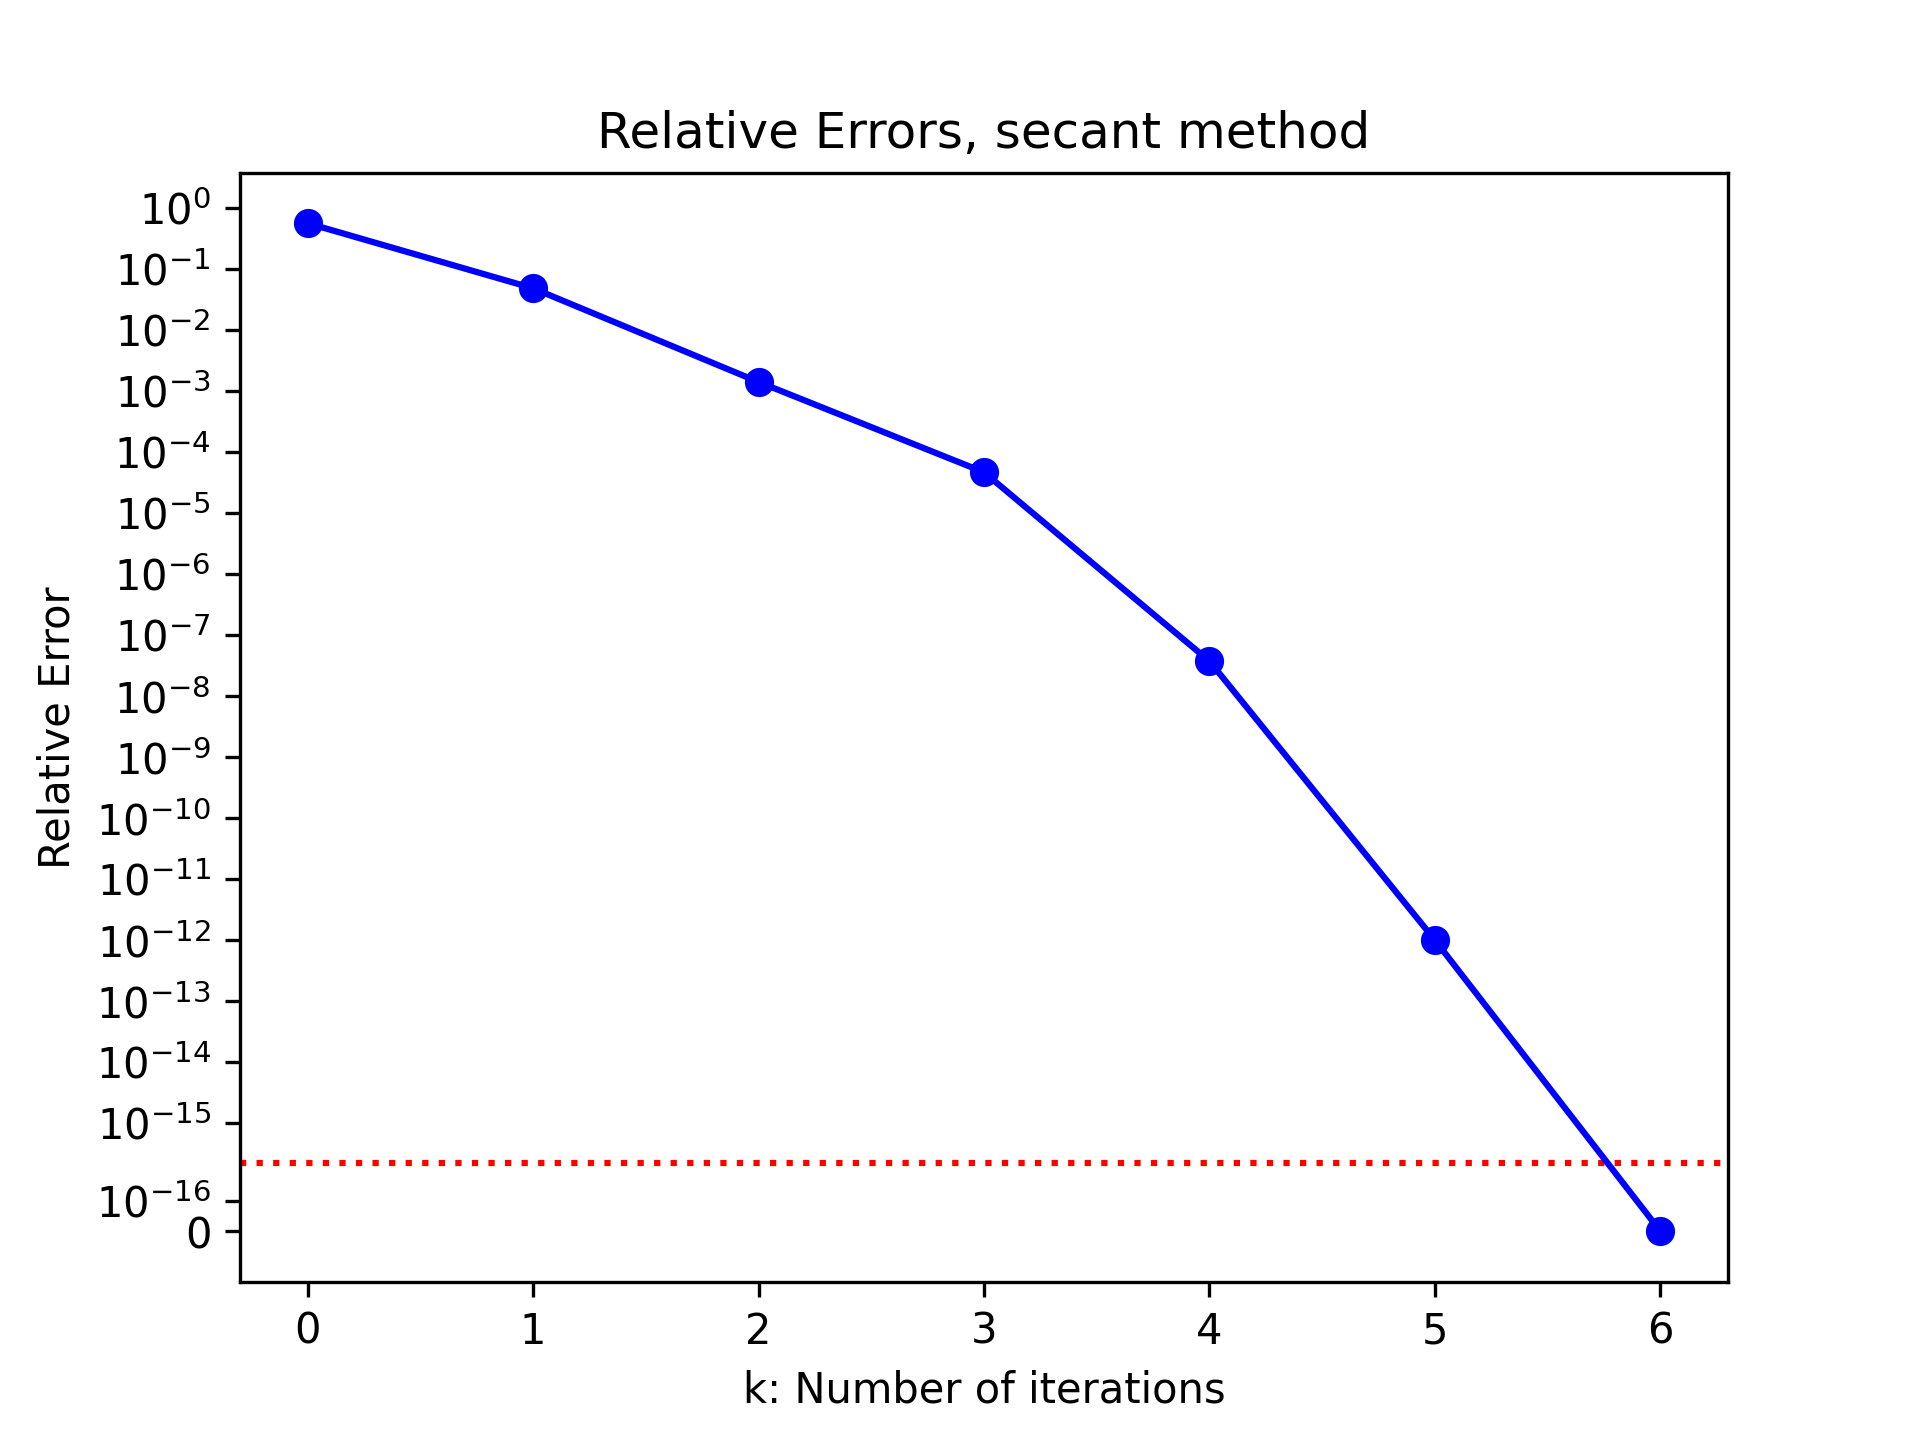
\includegraphics[scale=0.8]{./plots/secantrel.png}
    \caption{A matplotlib plot of the relative error of the Secant method}
\end{figure}


\subsection{Table (Ugly)}

We can import the table, as well.

\begin{figure}
    \centering
    \csvautotabular{./tables/secantrel.csv}
    \caption{A table of the relative error of the Secant method}
\end{figure}

\subsection{Table (Nice)}

And make a nice table.


\begin{figure}[h]
    \centering
    \begin{tabular}{|r|r|r|r|}\hline%
        $k$ & $x$ & $f(x)$ & \bfseries Rel. Error\\\hline\hline
        \csvreader[
            late after line = \\\hline,
            ]{./tables/secantrel.csv}%
            {k=\k, x=\x, f=\f, relerror=\relerror}%
            {\k & \x & \f & \relerror}%
        \end{tabular}
    \caption{A better looking table of the relative error of the Secant method}
\end{figure}

\end{document}
